\documentclass[9pt]{beamer}
\usepackage[french]{babel}
\usepackage[utf8]{inputenc}
\usepackage[T1]{fontenc}
\usepackage{minted}
%\usepackage{utopia} %font utopia imported
\usepackage{listings}
\usepackage{hyperref}
\usepackage{siunitx}
\usepackage{amsmath}
\usepackage{amssymb}
\usetheme{Madrid}
\usecolortheme{seagull}
\usefonttheme{structurebold}
\usepackage{booktabs} 
\usepackage{marvosym}
\usepackage{longtable}
\usepackage{tabularx}
\usepackage[autoplay]{animate}
\usepackage{graphics}
\usepackage{epstopdf}
\usepackage{pifont}
\usepackage{verbatim}
\newcommand{\executeiffilenewer}[3]{%
\ifnum\pdfstrcmp{\pdffilemoddate{#1}}%
{\pdffilemoddate{#2}}>0%
{\immediate\write18{#3}}\fi%
}
\newcommand{\includesvg}[1]{%
\executeiffilenewer{#1.svg}{#1.pdf}%
{inkscape -z -D --file=#1.svg %
--export-pdf=#1.pdf --export-latex}%
\input{#1}%
}
\DeclareUnicodeCharacter{202F}{\,}
\definecolor{mygreen}{HTML}{37980D}
\definecolor{myblue}{HTML}{0D089F}
\definecolor{myred}{HTML}{98290D}


\definecolor{vert}{RGB}{22,150,50}
\definecolor{vert2}{RGB}{170,230,130}

\definecolor{bleu}{RGB}{50,100,255}
\definecolor{bleu2}{RGB}{180,200,240}

\definecolor{orange}{RGB}{200,100,0}
\definecolor{orange2}{RGB}{240,190,70}

\definecolor{rouge}{RGB}{180,10,0}
\definecolor{rouge2}{RGB}{250,200,190}
\beamerboxesdeclarecolorscheme{objectif}{vert}{vert2}
\beamerboxesdeclarecolorscheme{idee}{bleu}{bleu2}
\beamerboxesdeclarecolorscheme{explication}{orange}{orange2}
\beamerboxesdeclarecolorscheme{propriete}{rouge}{rouge2}





%This block of code defines the information to appear in the
%Title page
\title[Formation d'Ingénieur en IA] %optional
{Réalisez le Cadrage}

\subtitle{d’un Projet IA}%~{\rm II}}

\author[Romain Boyrie] % (optional)
{R.~Boyrie}

\institute[OC - Msft] % (optional)
{
  Microsoft
  \and
  OpenClassrooms
}

\date[P11 juin 2022] % (optional)
{Projet \No 11, Juin 2022}


\logo{
\includegraphics[height=0.65cm]{../logo/logo}}

%End of title page configuration block
%------------------------------------------------------------

%------------------------------------------------------------
%The next block of commands puts the table of contents at the 
%beginning of each section and highlights the current section:

\AtBeginSection[]
{
  \begin{frame}
    \frametitle{Sommaire}
    \tableofcontents[currentsection]
  \end{frame}
}
%------------------------------------------------------------
%Montpellier dolphin
\expandafter\def\expandafter\insertshorttitle\expandafter{%
  \insertshorttitle\hfill%
  \insertframenumber\,/\,\inserttotalframenumber}

%\expandafter\def\expandafter\insertshorttitle\expandafter{% 
%\insertshorttitle\hfill\insertframenumber\,/\,\inserttotalframenumber}

\begin{document}

%The next statement creates the title page.
\frame{\titlepage}


%---------------------------------------------------------
%This block of code is for the table of contents after
%the title page
\begin{frame}
\frametitle{Sommaire}
\tableofcontents
\end{frame}
%---------------------------------------------------------

\section{Executive Summary}
\begin{frame}
	\frametitle{Executive Summary}
	\begin{figure}[!htb]
     \centering
     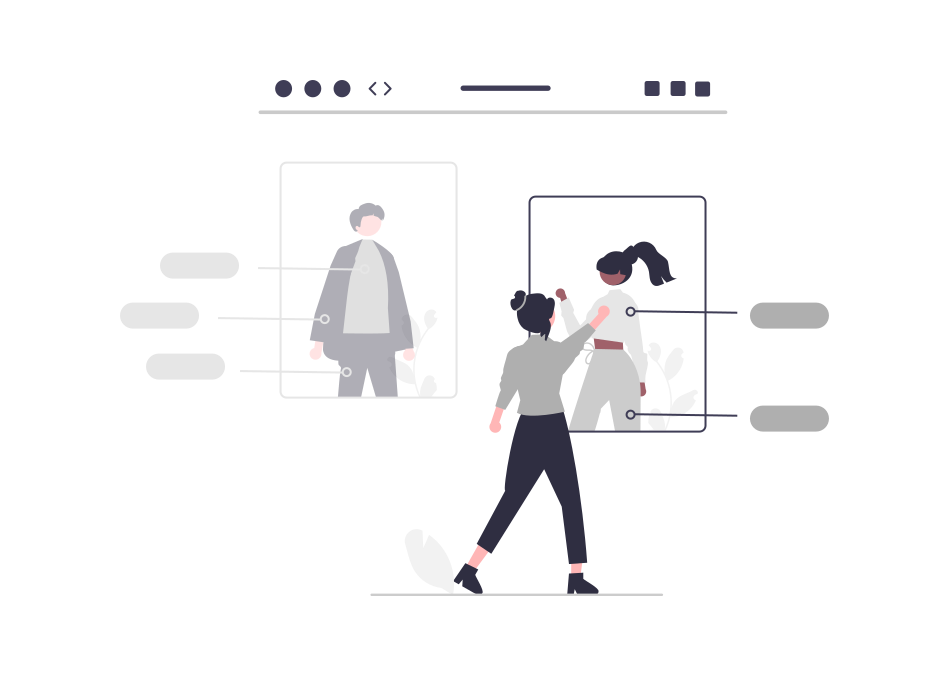
\includegraphics[width=.8\textwidth]{../media/Shopping}
   \label{Fig:shopping}
\end{figure}
\end{frame}
\begin{frame}
	\frametitle{Identification des RH, Techniques \& Financières}
	\begin{figure}[!htb]
     \centering
     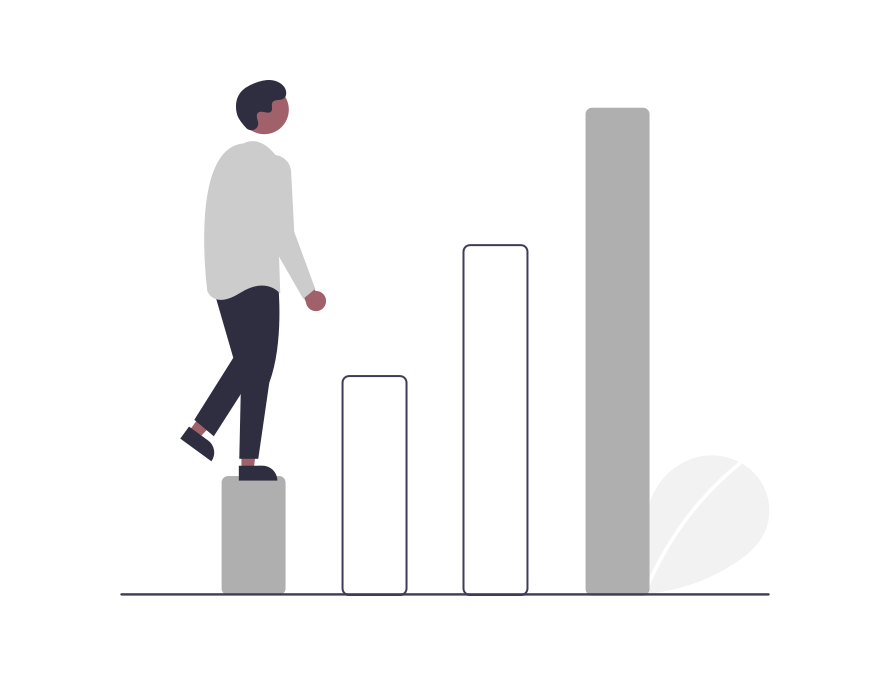
\includegraphics[width=.8\textwidth]{../media/stepping}
   \label{Fig:stepping}
\end{figure}
\end{frame}
\begin{frame}
	\frametitle{Optimisation des RH, Techniques \& Financières}
	En investissant un budget de départ, avec le pôle financier, nous avons :
\begin{figure}[!htb]
   \begin{minipage}{0.5\textwidth}
     \centering
     \begin{itemize} 
		\item[•] Calculer le fonds de roulement ;
      	\item[•] Le nombre de codeurs (3) ;
      	\begin{itemize}
      		\item[•] Développeur Web
      		\item[•] Data Scientist
      		\item[•] Administrateur 
      	\end{itemize}
     	\item[•] Le nombre de serveurs (14) ;
     	\item[•] Le dimensionnement des ressources (1.5k€/mois);
     	\item[•] Le retour sur investissement (30\%);
	 \end{itemize}	
   \end{minipage}\hfill
   \begin{minipage}{0.5\textwidth}
     \centering
     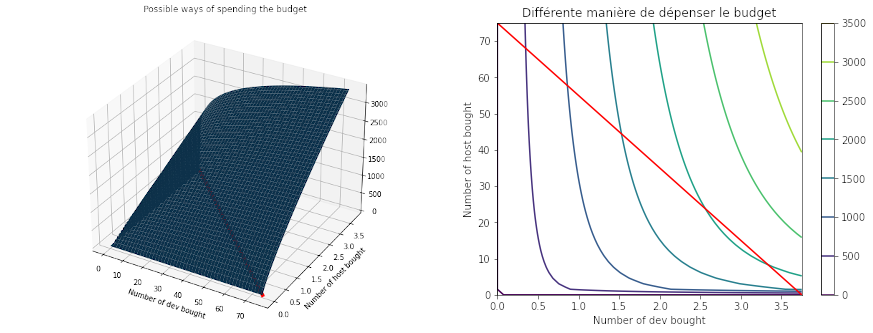
\includegraphics[width=1\linewidth]{../plots/optimisation}
     %\caption{Distribution en m}
     \label{Fig:optimisation}
   \end{minipage}
\end{figure}
\end{frame}

\begin{frame}
	\frametitle{Dimensionnement Technique}

\begin{table}[!ht]
\resizebox{.8\columnwidth}{!}{

    \centering
    \begin{tabular}{|l|l|l|l|}
    \hline
        Microsoft Azure Estimate & ~ & ~ & ~  \\ \hline
        Votre estimation & ~ & ~ & ~  \\ \hline
        Service type & Region & Description & Estimated monthly cost  \\ \hline
        Storage Accounts & West Europe & \parbox{9.5cm}{Redondance Stockage d’objets blob de bloc, Usage général v2, LRS, Niveau d’accès À chaud, 1 000 Go Capacité - À l'utilisation, 10 x 10 000 opérations d’écriture, 10 x 10 000 opérations de listage et de création de conteneur, 10 x 10 000 opérations de lecture, 100 000 opérations de lecture haute priorité Archive, 1 x 10 000 autres opérations. 1 000 Go Extraction de données, 1 000 Go Extraction de données haute priorité Archive, 1 000 Go Écriture de données} & €19,35  \\ \hline
        Azure SQL Database & West Europe & \parbox{9.5cm}{Base de données unique, LRS, vCore, Usage général, Provisionné, Série Standard (Gen 5), Redondance locale, 4 vCore, 1 instance(s) x 730Heures, Licence SQL (paiement à l’utilisation), 8 Go de stockage, 0 Go de stockage de sauvegarde, 5Go rétention à long terme} & €730,08  \\ \hline
        Azure Kubernetes Service (AKS) & West Europe & \parbox{9.5cm}{14 D2 v3 (2 processeurs virtuels, 8 Go de RAM) x 730 Heures (À l'utilisation), Linux ; 0 disques du système d’exploitation managés – S4, 2 clusters} & €1 281,42  \\ \hline
        Support & ~ & Support & €93,37  \\ \hline
        ~ & ~ & Licensing Program & Microsoft Customer Agreement (MCA) \\ \hline
        ~ & ~ & Billing Account & ~ \\ \hline
        ~ & ~ & Billing Profile & ~ \\ \hline
        ~ & ~ & Total & €2 124,22  \\ \hline
    \end{tabular}}
        \caption{Dimensionnement Technique}
    \label{dimension_tech}
\end{table}
\end{frame}


\section{Agile}
\begin{frame}
	\frametitle{Principes de la méthode Agile}
	\begin{figure}[!htb]
     \centering
     
\includegraphics[width=.7\textwidth]{../media/Schedule}
   \label{Fig:schedule}
\end{figure}
\end{frame}
\begin{frame}
	\frametitle{Agile}
	Les 12 principes d’Agile :
\begin{figure}[!htb]
   \begin{minipage}{0.7\textwidth}
     \centering
     \begin{enumerate}
  		\item Calculer le fonds de roulement ;
		\item Livrer dans les délais, pour satisfaire le client ;
		\item Adapter continuellement son offre au besoin du client ;
		\item Livraison fréquente, pour améliorer la qualité ;
		\item Coopérer en permanence avec le client ;
		\item Cadre de travail adapté, en équipe motivée ;
		\item Communiquer pour ne pas rompre le dialogue ;
		\item Mesurer l’avancée des travaux périodiquement ;
		\item Constance soutenable pour le rythme de travail ;
		\item Maîtrise technique et d’ouvrage ;
		\item Planifier des travaux courts, pour des fonctions simples ;
		\item Équipe organisée et responsable face au changement ;
		\item Accorder les rôles aux processus, pour maintenir la qualité.
	 \end{enumerate}	
   \end{minipage}\hfill
   \begin{minipage}{0.3\textwidth}
     \centering
     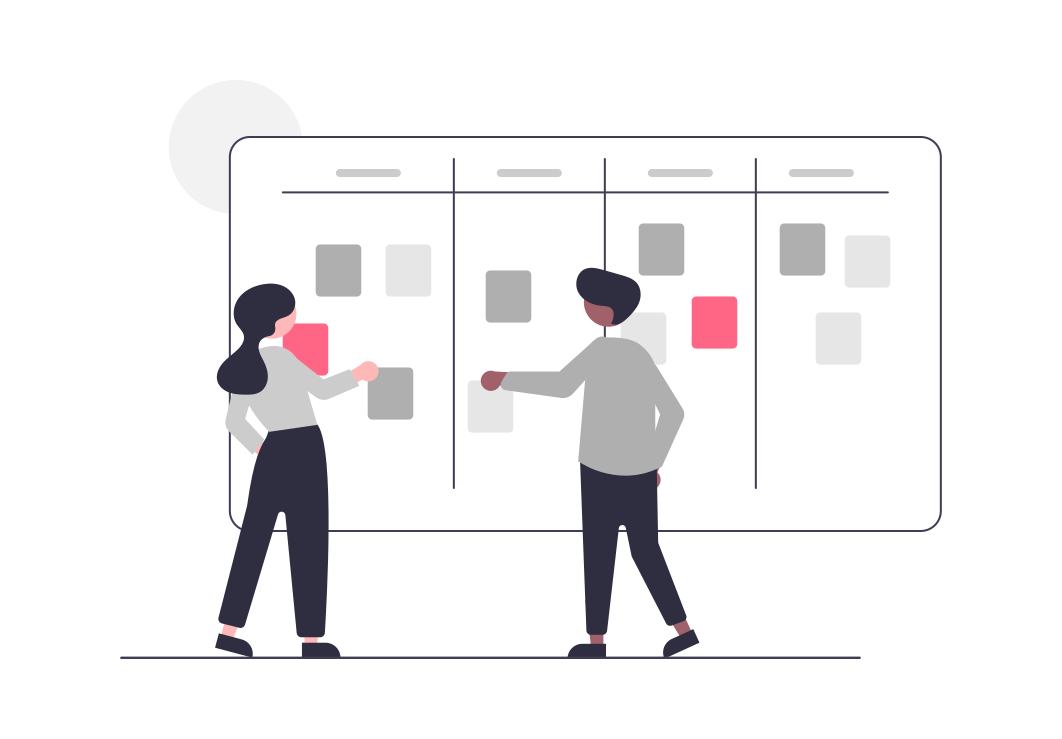
\includegraphics[width=1\linewidth]{../media/Scrum_board}
     %\caption{Distribution en m}
     \label{Fig:scrum_board}
   \end{minipage}
\end{figure}
\end{frame}
\begin{frame}
	\frametitle{Les Plus et les Moins de la Méthode Agile}
\begin{figure}[!htb]
   \begin{minipage}{0.7\textwidth}
    Les avantages de la méthode Agile :

     \begin{enumerate}
  		\item Améliore le contrôle entre le produit final et le besoin du client ;
		\item  La collaboration de personnes soutenues et motivées assure la qualité ;
		\item  L’engagement dans un objectif commun augmente la performance ;
		\item  Les tests accroissent la qualité du produit ;
		\item  Réduit les risques et améliore les coûts.
	 \end{enumerate}	
	Les inconvénients de la méthode Agile :
     \begin{enumerate}
  		\item  La Mauvaise application de la méthode par manque de compréhension ;
		\item  La réduction de la documentation dans le développement ;
		\item  La difficulté à adoper la culture que cela implique ;
		\item  La complexité de mise en place de la méthode pour les grandes entreprises.

	 \end{enumerate}		 	 
   \end{minipage}\hfill
   \begin{minipage}{0.3\textwidth}
     \centering
     \includegraphics[width=1\linewidth]{../media/Product_iteration}
     %\caption{Distribution en m}
     \label{Fig:product_iteration}
   \end{minipage}
\end{figure}
\end{frame}
\section{Backlog}
\begin{frame}
	\frametitle{Backlog}
	\begin{figure}[!htb]
     \centering
     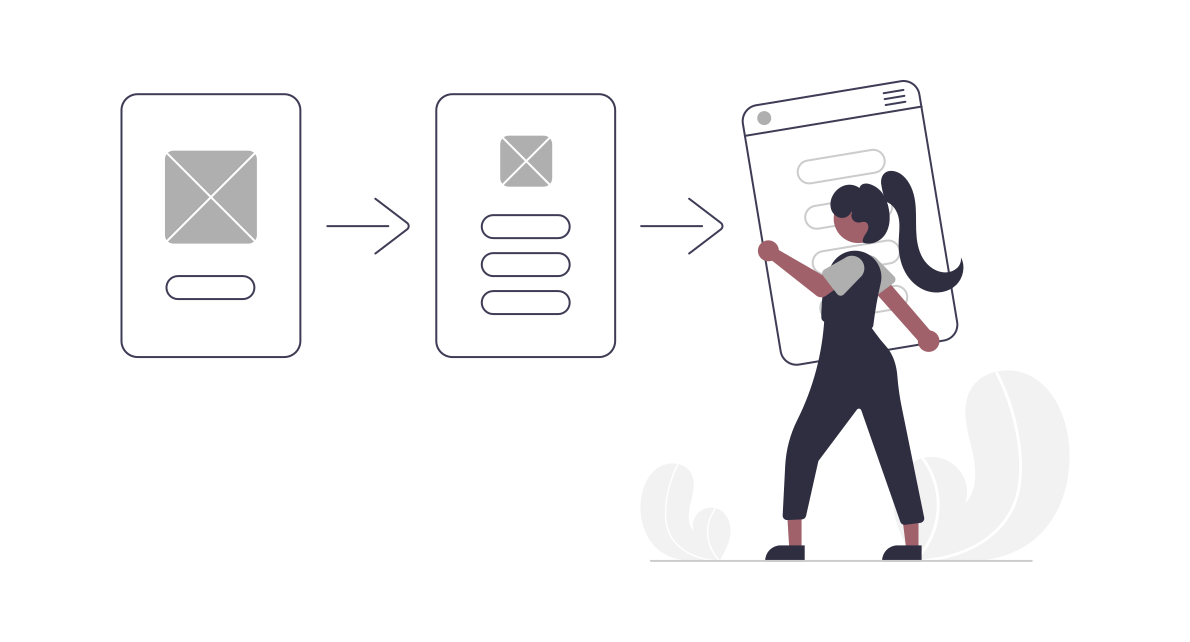
\includegraphics[width=.7\textwidth]{../media/User_flow}
   \label{Fig:user_flow}
\end{figure}
\end{frame}
\section{Mitigation des risques}
\begin{frame}
	\frametitle{Mitigation}
	\begin{figure}[!htb]
     \centering
     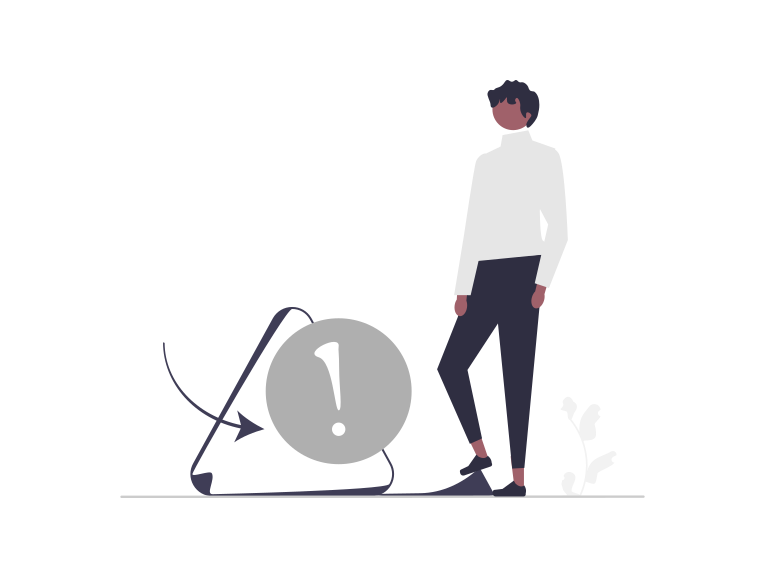
\includegraphics[width=.7\textwidth]{../media/Warning}
   \label{Fig:warning}
\end{figure}
\end{frame}
\section{Enjeux Légaux et Éthiques}
\begin{frame}
	\frametitle{Enjeux Légaux et Éthiques}
	\begin{figure}[!htb]
     \centering
     
\includegraphics[width=.8\textwidth]{../media/judge}
   \label{Fig:judge}
\end{figure}
\end{frame}
\begin{frame}
	\frametitle{Enjeux légaux}
\begin{figure}[!htb]
   \begin{minipage}{0.7\textwidth}
Cloud-computing (informatique dématérialisée)
La prestation est un contrat d’entreprise : 
\begin{itemize}

\item La clause objet
\item Obligations principales
\item Obligations accessoires
\item La clause de propriété intellectuelle
\item La clause de confidentialité
\item Les clauses et mesures de protection des données personnelles
\item La clause de réversibilité : possibilité du client de reprendre le contrôle sur l’outil
\item La clause de modification unilatérale du service : encadre les évolutions et mises-à-jours
\item La clause de loi applicable et de juridiction : droit applicable et juridiction compétente.

\end{itemize}	 
   \end{minipage}\hfill
   \begin{minipage}{0.3\textwidth}
     \centering
     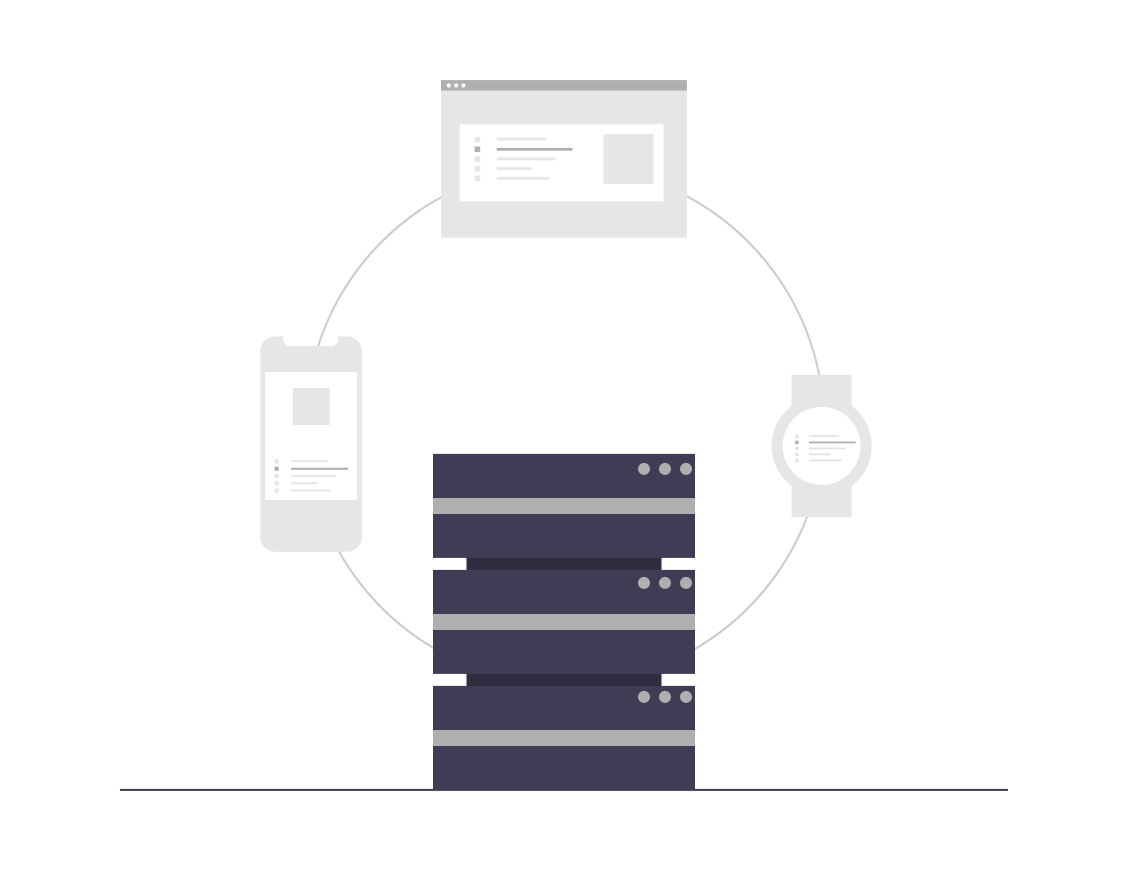
\includegraphics[width=1\linewidth]{../media/server_cluster}
     %\caption{Distribution en m}
     \label{Fig:server_cluster}
   \end{minipage}
\end{figure}
\end{frame}
\begin{frame}
	\frametitle{Enjeux éthique}
\begin{figure}[!htb]
   \begin{minipage}{0.7\textwidth}
La RGPD détaille que l’on doit retrouver a minima les éléments suivants :
\begin{itemize}
\item Une description systématique du traitement et de ses finalités, ainsi que la précision de l’intérêt légitime poursuivi ;
\item L’évaluation de la nécessité et de la proportionnalité du traitement par rapport aux finalités poursuivies ;
\item Une évaluation des risques pour les droits et libertés (des personnes physiques concernées) ;
\item Les mesures envisagées à cet égard, afin de protéger les données à caractère personnel.
\begin{enumerate}
\item Constituer un registre de vos traitements de données ;
\item Faire le tri dans vos données (pointer les données sensibles);
\item Respecter les droits des individus (politique de confidentialité);
\item Sécuriser vos données.
\end{enumerate}
\end{itemize}
 \end{minipage}\hfill
   \begin{minipage}{0.3\textwidth}
     \centering
     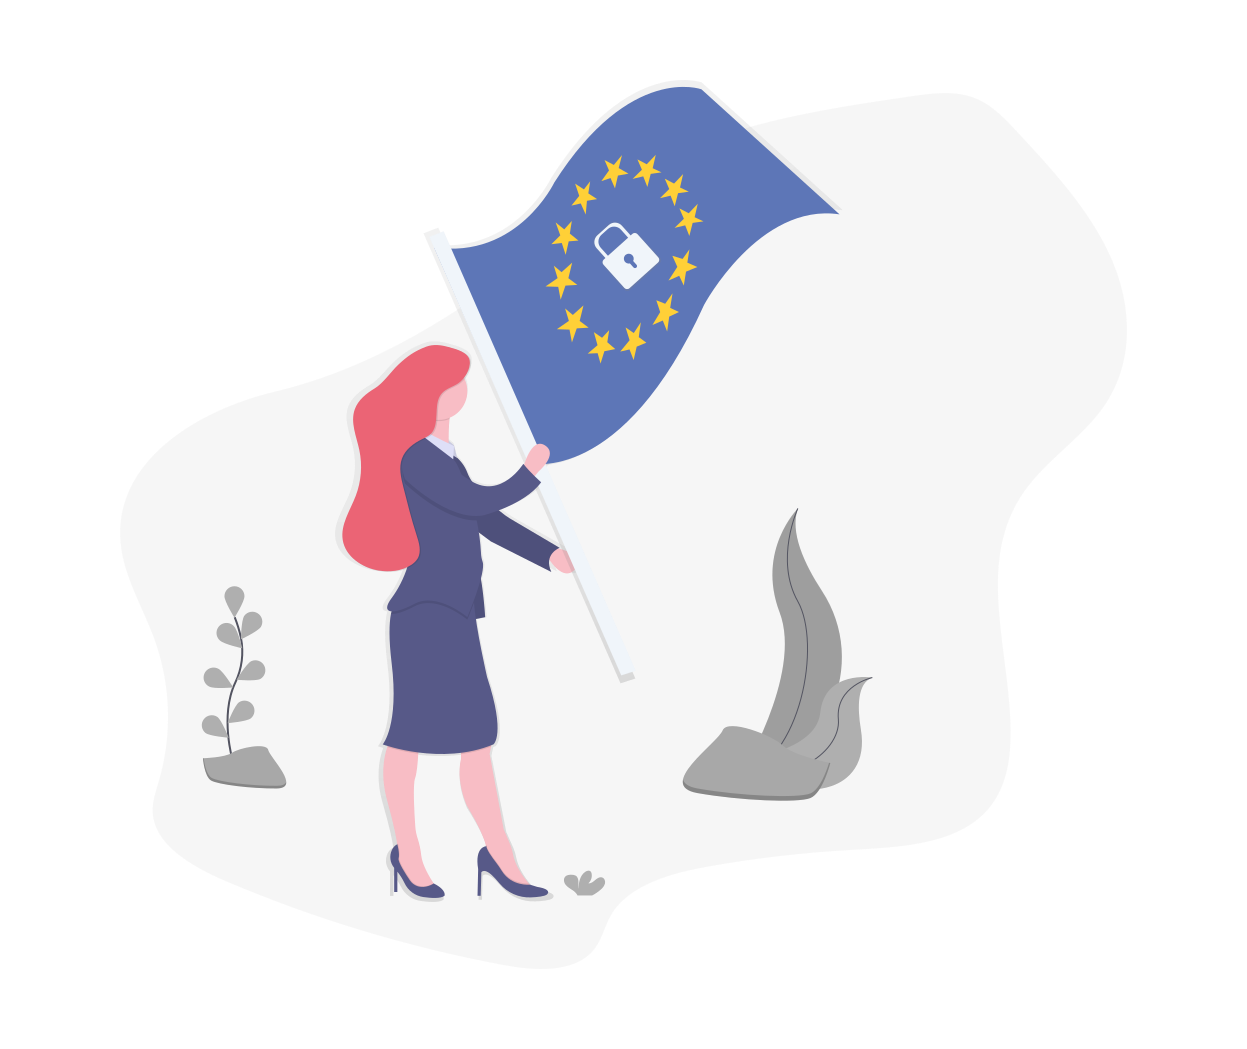
\includegraphics[width=1\linewidth]{../media/gdpr}
     %\caption{Distribution en m}
     \label{Fig:gdpr}
   \end{minipage}
\end{figure}
\end{frame}
\section{Conclusion}
\begin{frame}
	\frametitle{Conclusion}
	\begin{figure}[!htb]
     \centering
     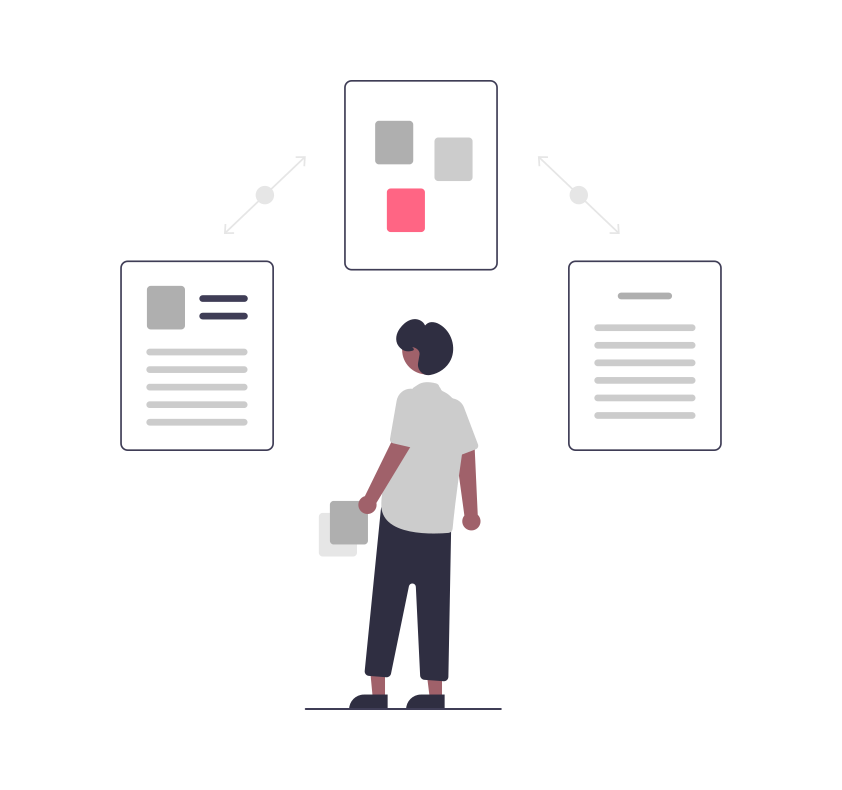
\includegraphics[width=.7\textwidth]{../media/Process}
   \label{Fig:process}
\end{figure}
\end{frame}
\begin{frame}
	\frametitle{Conclusion}
\begin{figure}[!htb]
   \begin{minipage}{0.6\textwidth}
Dans ce projet nous avons pu :
\begin{itemize}
\item Évaluer le profil financier du projet ;
\item Expliquer la méthode Agile SCRUM ;
\item Recenser les tâches et user stories du Backlog ;
\item Répertorier les actions préventives des risques ;
\item Détailler les enjeux légaux et éthiques ;

\end{itemize}
 \end{minipage}\hfill
   \begin{minipage}{0.4\textwidth}
     \centering
     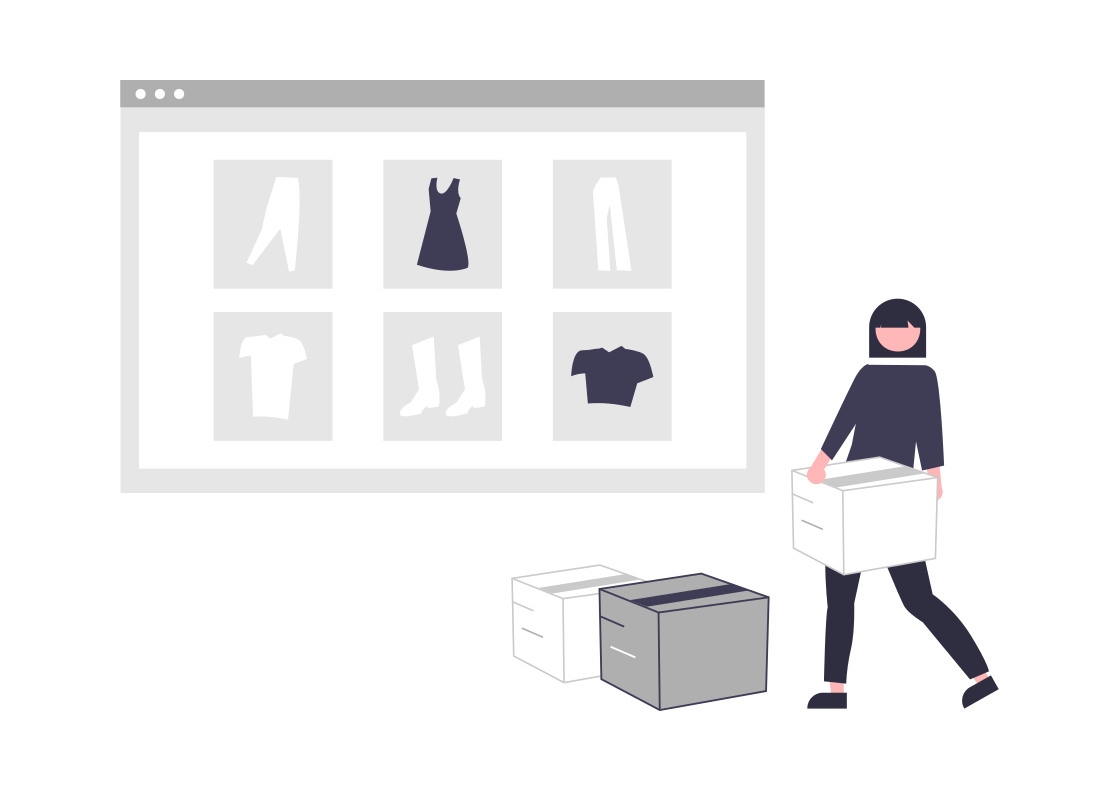
\includegraphics[width=1\linewidth]{../media/web_shopping}
     %\caption{Distribution en m}
     \label{Fig:web_shopping}
   \end{minipage}
\end{figure}
\end{frame}
\begin{frame}
	\frametitle{Fin}
	\begin{figure}[!htb]
     \centering
     
\includegraphics[width=.7\textwidth]{../media/appreciated}
   \label{Fig:appreciated}
\end{figure}
\end{frame}
\section{Annexe}
\begin{frame}
	\frametitle{Notebook Jupyter de l’Optimisation}
	\begin{figure}[!htb]
     \centering
     
\includegraphics[width=.7\textwidth]{../media/Lost_online}
   \label{Fig:lost_online}
\end{figure}
\end{frame}
\end{document}